\documentclass[twocolumn]{article}
\usepackage[utf8]{inputenc}
\usepackage[top=1in]{geometry}
\usepackage{graphicx}
\usepackage{hyperref}
% Calligraphic fonts
\newcommand{\calA}{{\cal A}}
\newcommand{\calB}{{\cal B}}
\newcommand{\calC}{{\cal C}}
\newcommand{\calD}{{\cal D}}
\newcommand{\calE}{{\cal E}}
\newcommand{\calF}{{\cal F}}
\newcommand{\calG}{{\cal G}}
\newcommand{\calH}{{\cal H}}
\newcommand{\calI}{{\cal I}}
\newcommand{\calJ}{{\cal J}}
\newcommand{\calK}{{\cal K}}
\newcommand{\calL}{{\cal L}}
\newcommand{\calM}{{\cal M}}
\newcommand{\calN}{{\cal N}}
\newcommand{\calO}{{\cal O}}
\newcommand{\calP}{{\cal P}}
\newcommand{\calQ}{{\cal Q}}
\newcommand{\calR}{{\cal R}}
\newcommand{\calS}{{\cal S}}
\newcommand{\calT}{{\cal T}}
\newcommand{\calU}{{\cal U}}
\newcommand{\calV}{{\cal V}}
\newcommand{\calW}{{\cal W}}
\newcommand{\calX}{{\cal X}}
\newcommand{\calY}{{\cal Y}}
\newcommand{\calZ}{{\cal Z}}

% Sets:
\newcommand{\setA}{\textsf{A}}
\newcommand{\setB}{\textsf{B}}
\newcommand{\setC}{\textsf{C}}
\newcommand{\setD}{\textsf{D}}
\newcommand{\setE}{\textsf{E}}
\newcommand{\setF}{\textsf{F}}
\newcommand{\setG}{\textsf{G}}
\newcommand{\setH}{\textsf{H}}
\newcommand{\setI}{\textsf{I}}
\newcommand{\setJ}{\textsf{J}}
\newcommand{\setK}{\textsf{K}}
\newcommand{\setL}{\textsf{L}}
\newcommand{\setM}{\textsf{M}}
\newcommand{\setN}{\textsf{N}}
\newcommand{\setO}{\textsf{O}}
\newcommand{\setP}{\textsf{P}}
\newcommand{\setQ}{\textsf{Q}}
\newcommand{\setR}{\textsf{R}}
\newcommand{\setS}{\textsf{S}}
\newcommand{\setT}{\textsf{T}}
\newcommand{\setU}{\textsf{U}}
\newcommand{\setV}{\textsf{V}}
\newcommand{\setW}{\textsf{W}}
\newcommand{\setX}{\textsf{X}}
\newcommand{\setY}{\textsf{Y}}
\newcommand{\setZ}{\textsf{Z}}

% Vectors
\newcommand{\bfa}{\mathbf{a}}
\newcommand{\bfb}{\mathbf{b}}
\newcommand{\bfc}{\mathbf{c}}
\newcommand{\bfd}{\mathbf{d}}
\newcommand{\bfe}{\mathbf{e}}
\newcommand{\bff}{\mathbf{f}}
\newcommand{\bfg}{\mathbf{g}}
\newcommand{\bfh}{\mathbf{h}}
\newcommand{\bfi}{\mathbf{i}}
\newcommand{\bfj}{\mathbf{j}}
\newcommand{\bfk}{\mathbf{k}}
\newcommand{\bfl}{\mathbf{l}}
\newcommand{\bfm}{\mathbf{m}}
\newcommand{\bfn}{\mathbf{n}}
\newcommand{\bfo}{\mathbf{o}}
\newcommand{\bfp}{\mathbf{p}}
\newcommand{\bfq}{\mathbf{q}}
\newcommand{\bfr}{\mathbf{r}}
\newcommand{\bfs}{\mathbf{s}}
\newcommand{\bft}{\mathbf{t}}
\newcommand{\bfu}{\mathbf{u}}
\newcommand{\bfv}{\mathbf{v}}
\newcommand{\bfw}{\mathbf{w}}
\newcommand{\bfx}{\mathbf{x}}
\newcommand{\bfy}{\mathbf{y}}
\newcommand{\bfz}{\mathbf{z}}


\newcommand{\bfalpha}{\boldsymbol{\alpha}}
\newcommand{\bfbeta}{\boldsymbol{\beta}}
\newcommand{\bfgamma}{\boldsymbol{\gamma}}
\newcommand{\bfdelta}{\boldsymbol{\delta}}
\newcommand{\bfepsilon}{\boldsymbol{\epsilon}}
\newcommand{\bfzeta}{\boldsymbol{\zeta}}
\newcommand{\bfeta}{\boldsymbol{\eta}}
\newcommand{\bftheta}{\boldsymbol{\theta}}
\newcommand{\bfiota}{\boldsymbol{\iota}}
\newcommand{\bfkappa}{\boldsymbol{\kappa}}
\newcommand{\bflambda}{\boldsymbol{\lambda}}
\newcommand{\bfmu}{\boldsymbol{\mu}}
\newcommand{\bfnu}{\boldsymbol{\nu}}
\newcommand{\bfomicron}{\boldsymbol{\omicron}}
\newcommand{\bfpi}{\boldsymbol{\pi}}
\newcommand{\bfrho}{\boldsymbol{\rho}}
\newcommand{\bfsigma}{\boldsymbol{\sigma}}
\newcommand{\bftau}{\boldsymbol{\tau}}
\newcommand{\bfupsilon}{\boldsymbol{\upsilon}}
\newcommand{\bfphi}{\boldsymbol{\phi}}
\newcommand{\bfchi}{\boldsymbol{\chi}}
\newcommand{\bfpsi}{\boldsymbol{\psi}}
\newcommand{\bfomega}{\boldsymbol{\omega}}
\newcommand{\bfxi}{\boldsymbol{\xi}}
\newcommand{\bfell}{\boldsymbol{\ell}}

% Matrices
\newcommand{\bfA}{\mathbf{A}}
\newcommand{\bfB}{\mathbf{B}}
\newcommand{\bfC}{\mathbf{C}}
\newcommand{\bfD}{\mathbf{D}}
\newcommand{\bfE}{\mathbf{E}}
\newcommand{\bfF}{\mathbf{F}}
\newcommand{\bfG}{\mathbf{G}}
\newcommand{\bfH}{\mathbf{H}}
\newcommand{\bfI}{\mathbf{I}}
\newcommand{\bfJ}{\mathbf{J}}
\newcommand{\bfK}{\mathbf{K}}
\newcommand{\bfL}{\mathbf{L}}
\newcommand{\bfM}{\mathbf{M}}
\newcommand{\bfN}{\mathbf{N}}
\newcommand{\bfO}{\mathbf{O}}
\newcommand{\bfP}{\mathbf{P}}
\newcommand{\bfQ}{\mathbf{Q}}
\newcommand{\bfR}{\mathbf{R}}
\newcommand{\bfS}{\mathbf{S}}
\newcommand{\bfT}{\mathbf{T}}
\newcommand{\bfU}{\mathbf{U}}
\newcommand{\bfV}{\mathbf{V}}
\newcommand{\bfW}{\mathbf{W}}
\newcommand{\bfX}{\mathbf{X}}
\newcommand{\bfY}{\mathbf{Y}}
\newcommand{\bfZ}{\mathbf{Z}}


\newcommand{\bfGamma}{\boldsymbol{\Gamma}}
\newcommand{\bfDelta}{\boldsymbol{\Delta}}
\newcommand{\bfTheta}{\boldsymbol{\Theta}}
\newcommand{\bfLambda}{\boldsymbol{\Lambda}}
\newcommand{\bfPi}{\boldsymbol{\Pi}}
\newcommand{\bfSigma}{\boldsymbol{\Sigma}}
\newcommand{\bfUpsilon}{\boldsymbol{\Upsilon}}
\newcommand{\bfPhi}{\boldsymbol{\Phi}}
\newcommand{\bfPsi}{\boldsymbol{\Psi}}
\newcommand{\bfOmega}{\boldsymbol{\Omega}}


% Blackboard Bold:
\newcommand{\bbA}{\mathbb{A}}
\newcommand{\bbB}{\mathbb{B}}
\newcommand{\bbC}{\mathbb{C}}
\newcommand{\bbD}{\mathbb{D}}
\newcommand{\bbE}{\mathbb{E}}
\newcommand{\bbF}{\mathbb{F}}
\newcommand{\bbG}{\mathbb{G}}
\newcommand{\bbH}{\mathbb{H}}
\newcommand{\bbI}{\mathbb{I}}
\newcommand{\bbJ}{\mathbb{J}}
\newcommand{\bbK}{\mathbb{K}}
\newcommand{\bbL}{\mathbb{L}}
\newcommand{\bbM}{\mathbb{M}}
\newcommand{\bbN}{\mathbb{N}}
\newcommand{\bbO}{\mathbb{O}}
\newcommand{\bbP}{\mathbb{P}}
\newcommand{\bbQ}{\mathbb{Q}}
\newcommand{\bbR}{\mathbb{R}}
\newcommand{\bbS}{\mathbb{S}}
\newcommand{\bbT}{\mathbb{T}}
\newcommand{\bbU}{\mathbb{U}}
\newcommand{\bbV}{\mathbb{V}}
\newcommand{\bbW}{\mathbb{W}}
\newcommand{\bbX}{\mathbb{X}}
\newcommand{\bbY}{\mathbb{Y}}
\newcommand{\bbZ}{\mathbb{Z}}




\title{ECE 417/598: Homework 1}
\author{Max marks: 120}
\date{Due on Jan 28, 2021, before class.}
\newtheorem{prob}{Problem}

\newcommand{\bx}{\bar{x}}
\newcommand{\by}{\bar{y}}
\newcommand{\bz}{\bar{z}}
\begin{document}

\maketitle

You are allowed to use any matrix or linear algebra library (Eigen or xtensor), but no
library that implements rotation matrices. You are not allowed to use
Eigen/Geometry. You can use the following code for generating random rotation matrices:
\href{https://github.com/wecacuee/ECE417-Mobile-Robots/blob/master/notebooks/random_rotation.cpp}{random\_rotation.cpp}.

\section{Jan 21 Lecture}
\begin{prob}
  Degrees of Freedom of a quantity is the number independent scalar variables
  needed to represent that quantity. What is degrees of freedom required to 
  \begin{enumerate}
    \item Position and orientation in 1-D
    \item Position and orientation in 2-D
    \item Position and orientation in 3-D
    \item Position and orientation in 4-D
  \end{enumerate} (8 marks. Estimated time: 15 min)
  Justify your answer.
\end{prob}

\begin{prob}
  Write a program in C++ that checks if a given
  3x3 matrix is a valid Rotation matrix is a valid Rotation matrix  (check for
  orthonormality i.e. orthogonality and determinant = 1). You may use Eigen's
  matrix multiplication and determinant() function. (10 marks. Used in the
  following problems. Estimated time: 15 min). 
\end{prob}

\begin{prob}
  Write a pair of functions in C++ that converts rotation matrix from XYZ Euler
angles (roll, pitch, yaw) and vice versa. Test the pair of functions with
randomly generated Euler angles. And check if the converted rotation matrix is
orthonormal. What happens when pitch = $\pi/2$, are you able to convert from
rotation matrix to Euler angle? Why or why not? (50 marks. Estimated time: 30 min)
\end{prob}

\begin{prob}
  Write a pair of functions in C++ that converts rotation
  matrix from axis-angle format and vice-versa. Test the pair of functions with randomly
  generated axis-angle representation. And check if the converted rotation
  matrix  is orthonormal. (50 marks. Estimated time: 30 min)
\end{prob}

\begin{prob}
  Write a function in C++ that generates a 4x4 transformation given axis-angle
  representation and translation. (20 marks. Estimated time: 15 min).
\end{prob}

\begin{prob}
  For the given robot write down the axis-angle rotation from joint to joint
  assuming the joint angles to be  $\theta_1$, $\theta_2$, $\theta_3$ respectively.
  \\
  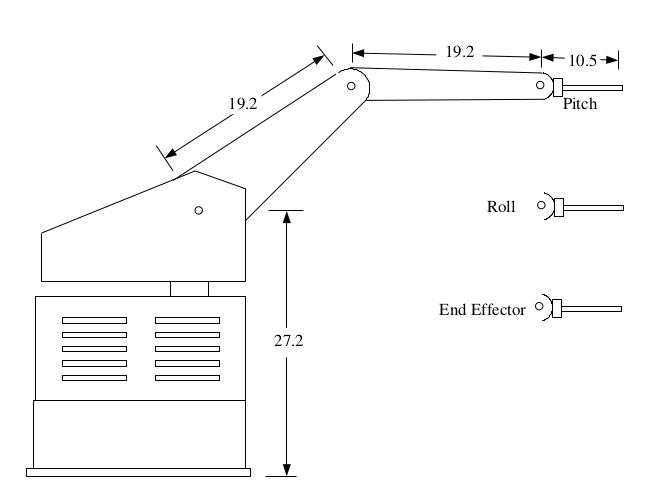
\includegraphics[width=\linewidth]{robot.png}
  \\
\end{prob}

\section{Jan 24 Lecture}
\begin{prob}
  The following is known about a smooth trajectory: p(0) = 0, v(0) = 0, 
  p(3) = 2, p(7) = 0, v(7) = 0 and velocity and acceleration are 
  continuous everywhere.  

  \begin{enumerate}
  \item What is the lowest degree single polynomial which could be used?  
  \item Give two advantages to using a spline curve instead. 
  \item What degree polynomials would you suggest for the splines?  
  \item Write the polynomials.  
  \item Write the set of equations which would be used to solve for the coefficients. Do not use normalized time. 
  \item Solve for the coefficients.
  \item Write the set of equations which would be used to solve for the coefficients. Use normalized time. 
  \item Solve for the coefficients.
  \end{enumerate}
\end{prob}


\bibliography{main}
\bibliographystyle{plain}
\end{document}
